% !TEX root = Tesi.tex
\chead{}
\chapter{Combining approaches}

The evolution of the Internet and the amount of data available from web usage mining and IoT devices has led to an enormous proliferation of the accessible information as per described in the previous sections.  In this chapter, we focus on the actual process of modeling the collected behavioral data from these two sources, the analysis of the associated log records and the discovery of usage patterns with the goal of addressing some of the weaknesses of the standard approaches for web personalization.

Before we can efficiently represent content visualized on user interfaces, navigation paths and user-triggered events on a web application, we need to take a little detour describing a standard modeling language capable of modeling such interactions in detail.

\section{The IFML language}

The Interaction Flow Modeling Language (IFML)\cite{IFML-1, IFML-2} is designed for describing and controlling the behavior of front-end software applications, it brings several advantages to the development process such as promoting the separation of concerns between roles and increasing the overall understanding of the product for non-technical stakeholders. To achieve so IFML supports formal specification for interface composition, user interaction and event management independently of the implementation platform and it was adopted as a standard by the Object Management Group (OMG) in March 2013.

IFML supports the following concepts: 

\begin{itemize}
  \item \textbf{The view structure} describes \textit{ViewContainers}, their nesting relationships, their visibility and their reachability.
    
  \item \textbf{The view content} manages \textit{ViewComponents}, i.e., content and data entry elements contained within ViewContainers.
  
  \item \textbf{The events} defines the \textit{Events} that may affect the state of the user interface. \textit{Events} can be produced by the user’s interaction, by the application, or by an external system; 

  \item \textbf{The actions} triggered by the user’s events. The effect of an \textit{Event} is represented by an \textit{InteractionFlow} connection, which connects the event to the \textit{ViewContainer} or \textit{ViewComponent} affected by the \textit{Event}. The \textit{InteractionFlow} expresses a change of state of the user interface: the occurrence of the event triggers a change in the state that produces a transition in the user interface.
  
  \item \textbf{The navigation flow} indicates the effect of an Event on the user interface.

  \item \textbf{The data flow} indicates the data passed between \textit{ViewComponents} and \textit{Actions}
  
  \item \textbf{The parameter binding} illustrates the input-output dependencies between \textit{ViewComponents} and between \textit{ViewComponents} and \textit{Actions}. 


\end{itemize} 

\vspace{0.5cm}
\begin{figure}[H]
  \centering
    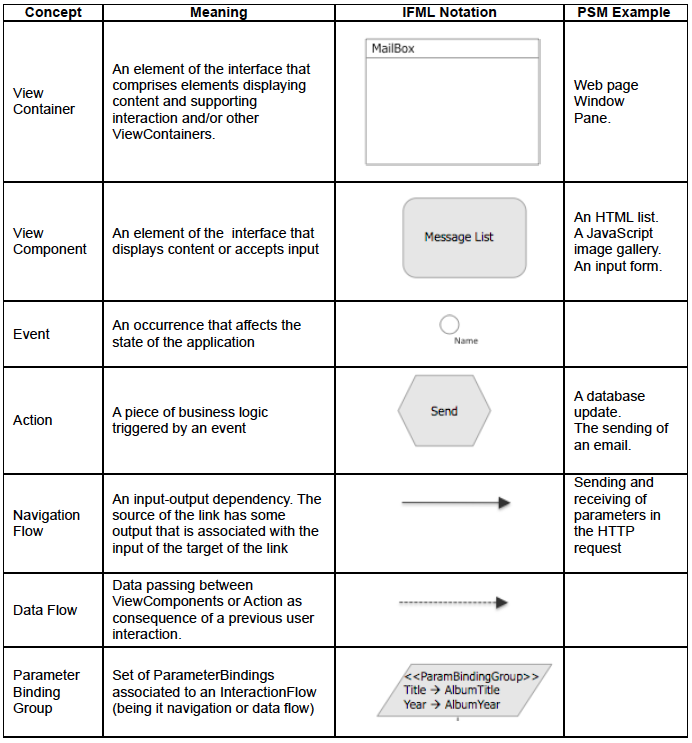
\includegraphics[width=10cm]{images/ifml.jpg}
  \caption{Main IFML concepts and notations.}
  \label{fig:ifml}
\end{figure}
\vspace{0.5cm}

\newpage

\section{Navigational modeling for the Web}

eCommerce website front ends are usually built using shared and reusable components (forms, list views, detail views, etc.) which have a specific and expected behavior.
For example, Product lists and grids show record details for the user to view and interact with an action on these, "Add To Cart" call-to-action buttons are presented within product pages to trigger a different response and so on.
All these interactive operations can be represented using the IFML notation.

To demonstrate the versatility and adaptability of this modeling language we introduce a real-life example which we will use as a reference from this chapter forward: an online boutique website called \textit{"Madison Island"} specialized in fashion items running on an eCommerce platform.

Madison Island presents all the features of a typical eCommerce digital store including navigation and browsing of its catalog, product searching, customer account section, shopping cart and order processing. 


\vspace{0.1cm}
\begin{figure}[htbp]
  \centering
    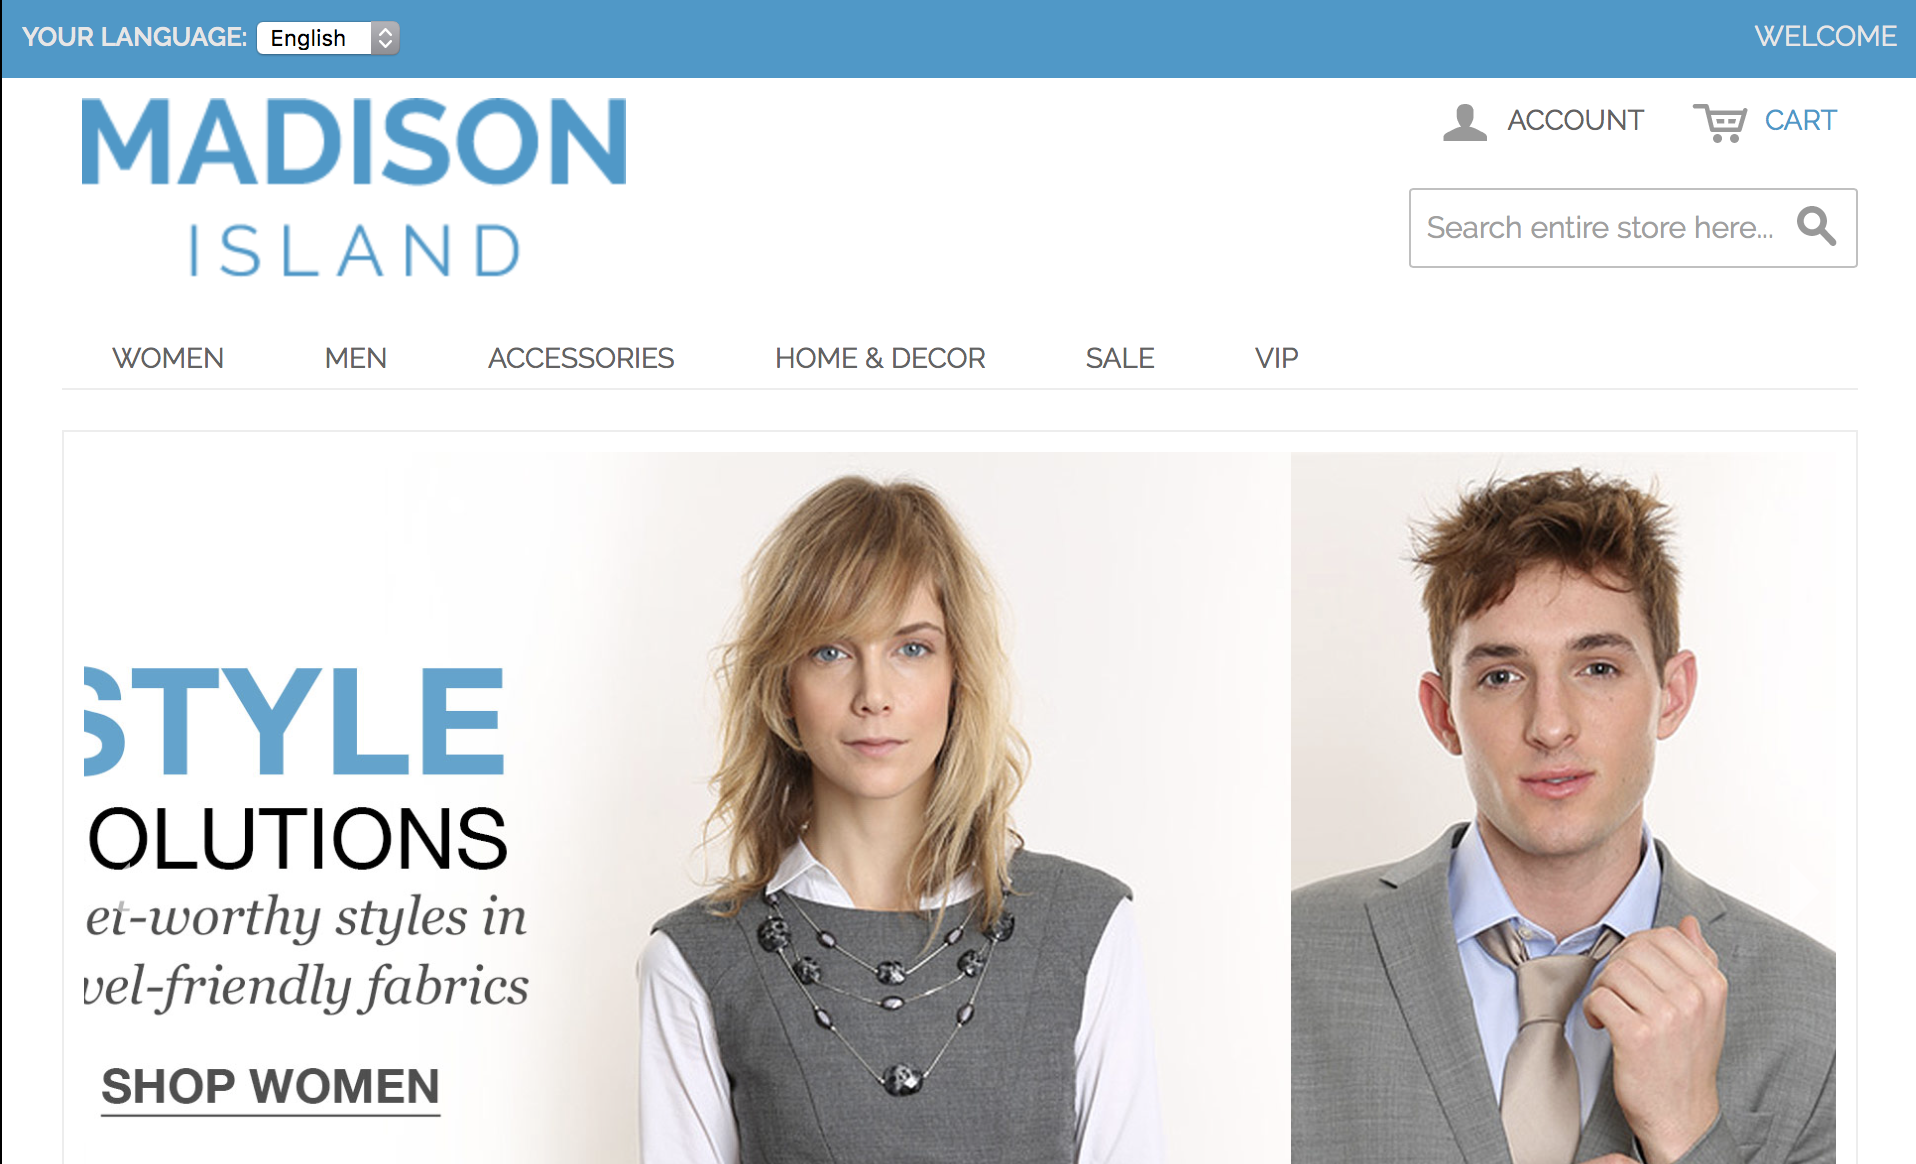
\includegraphics[width=12cm]{images/home.png}
  \caption{Madison Island digital store homepage}
  \label{fig:home}
\end{figure}
\vspace{0.1cm}


Figure \ref{fig:home} shows the home page of the website. In this section, the user can select one of the product categories, access his customer area, switch the language of the website, search for an item or go directly to the shopping cart. 

In the following subsections, we analyze a couple of scenarios related to users navigational behaviors exposing both their representation in IFML notation and the associated server log entries in the application server.

\newpage
\subsection{The product page journey}

Starting from the homepage the user can interact with the navigation menu to select from a set of categories available.  (Figure \ref{fig:navigation})

\vspace{0.1cm}
\begin{figure}[H]
  \centering
    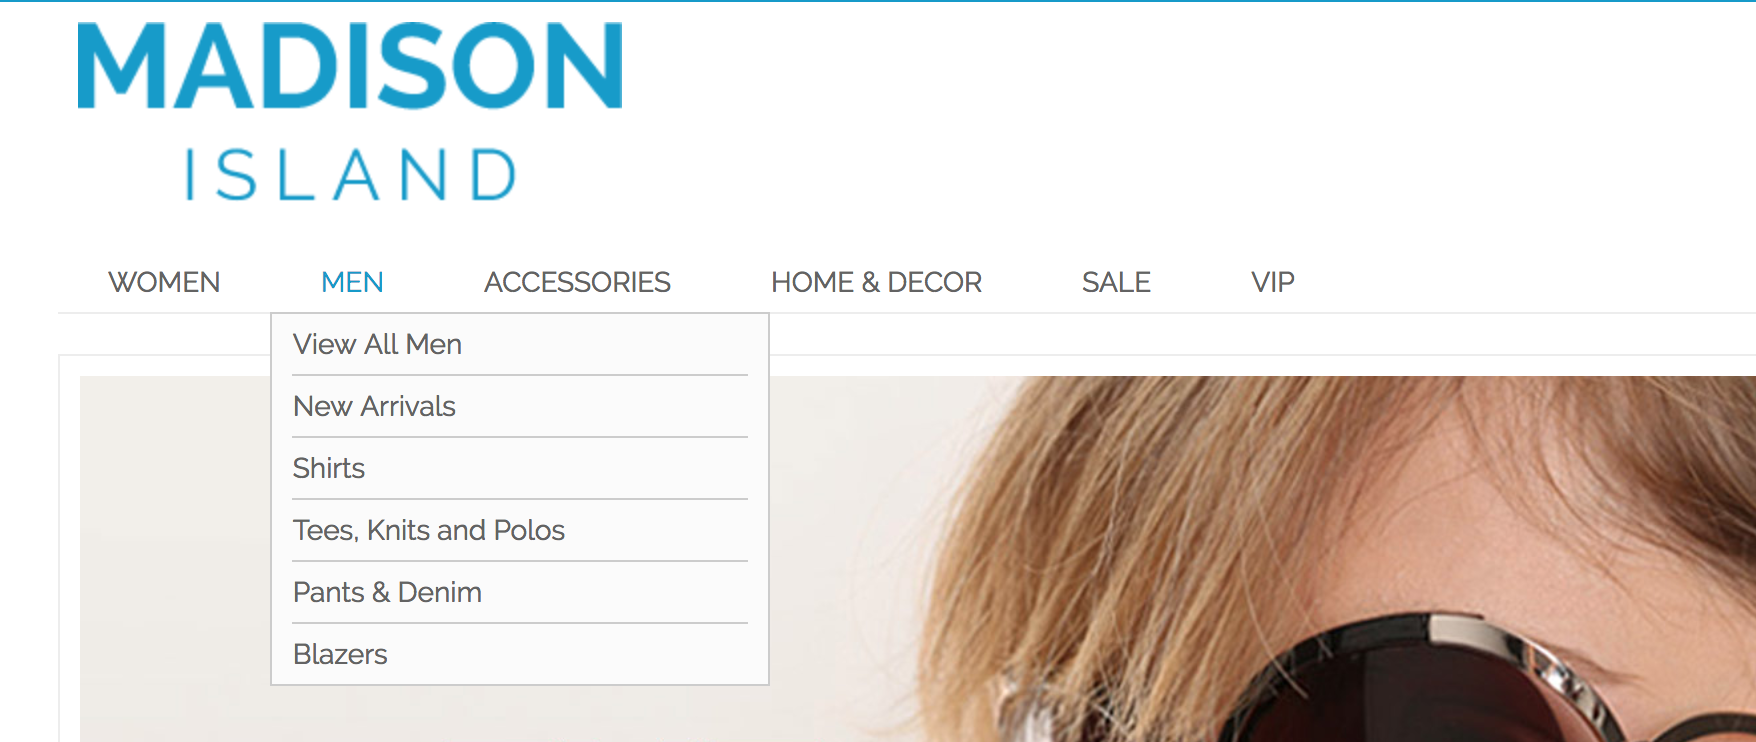
\includegraphics[width=9cm]{images/madison/navigation.png}
  \caption{Navigation menu}
  \label{fig:navigation}
\end{figure}
\vspace{0.1cm}

Depending on the category display mode, a category page can either list CMS content showing a list of links to children categories serving as an intermediary transitional page or directly present its products to the user.
(Figure \ref{fig:category-display-modes})


\vspace{0.1cm}
\begin{figure}[H]
  \centering
  \subfloat[Category listing]{{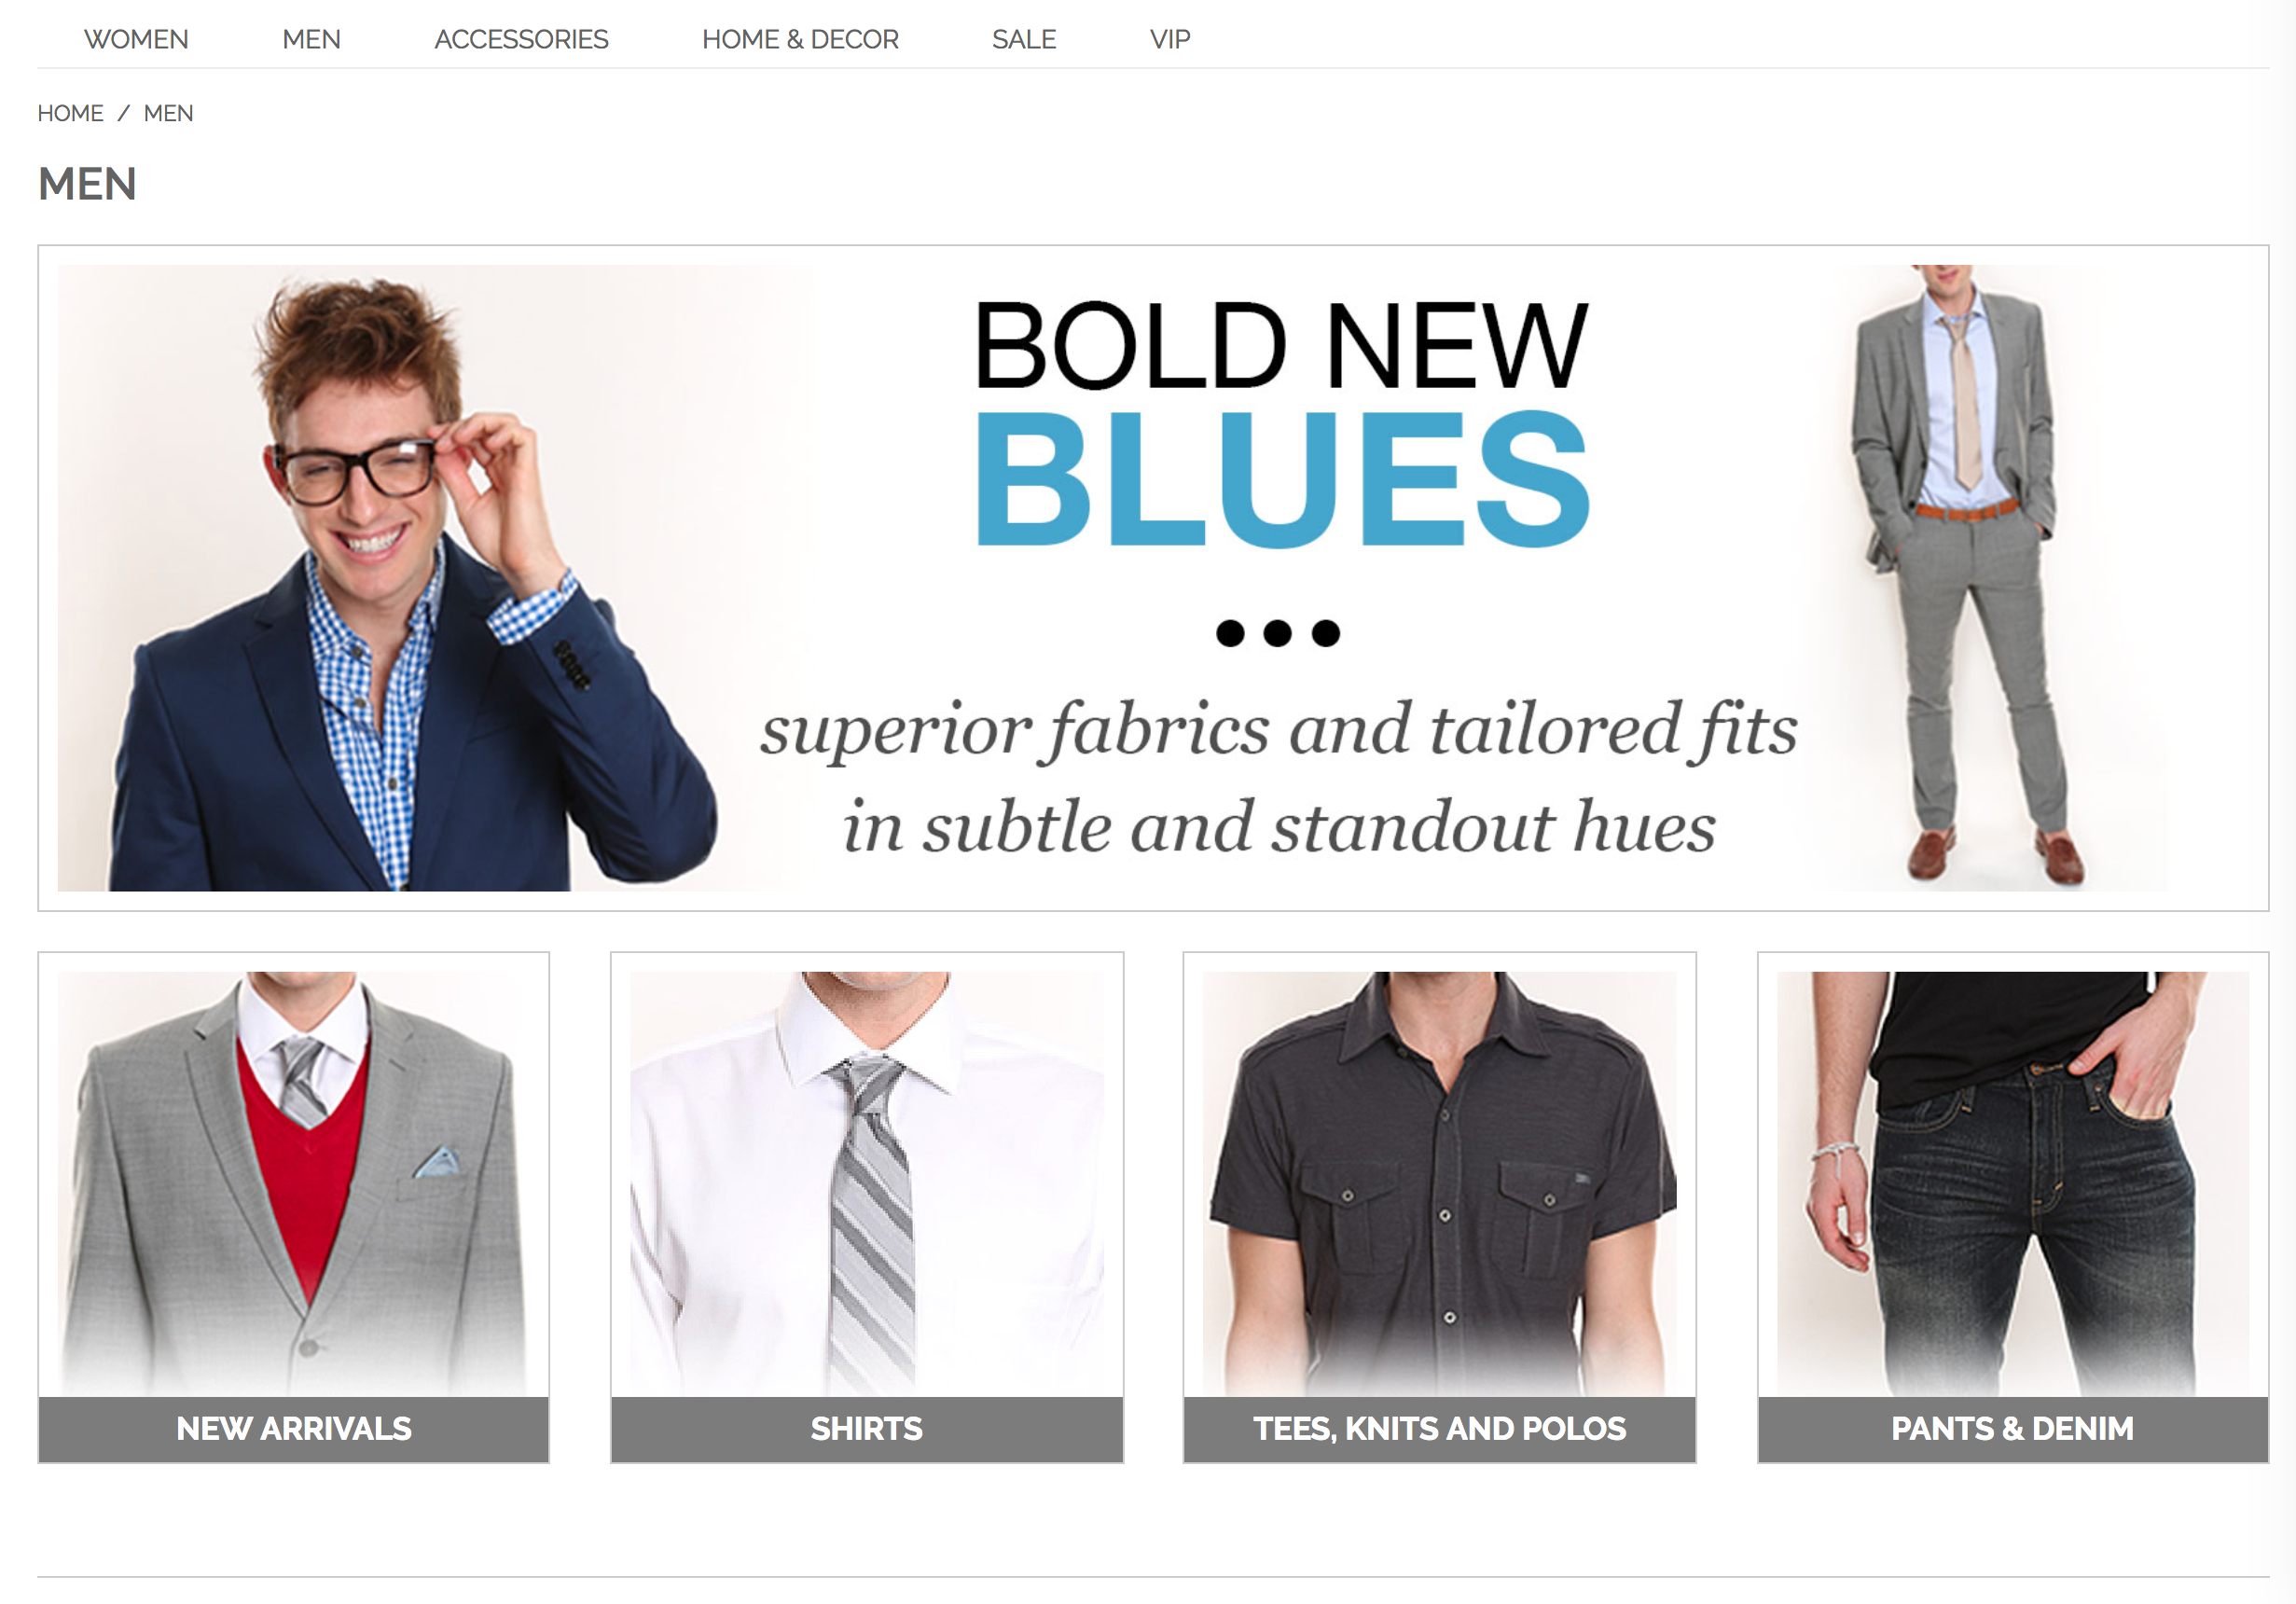
\includegraphics[width=7cm]{images/madison/category-cms.png} }}%
  \qquad
  \subfloat[Product listing]{{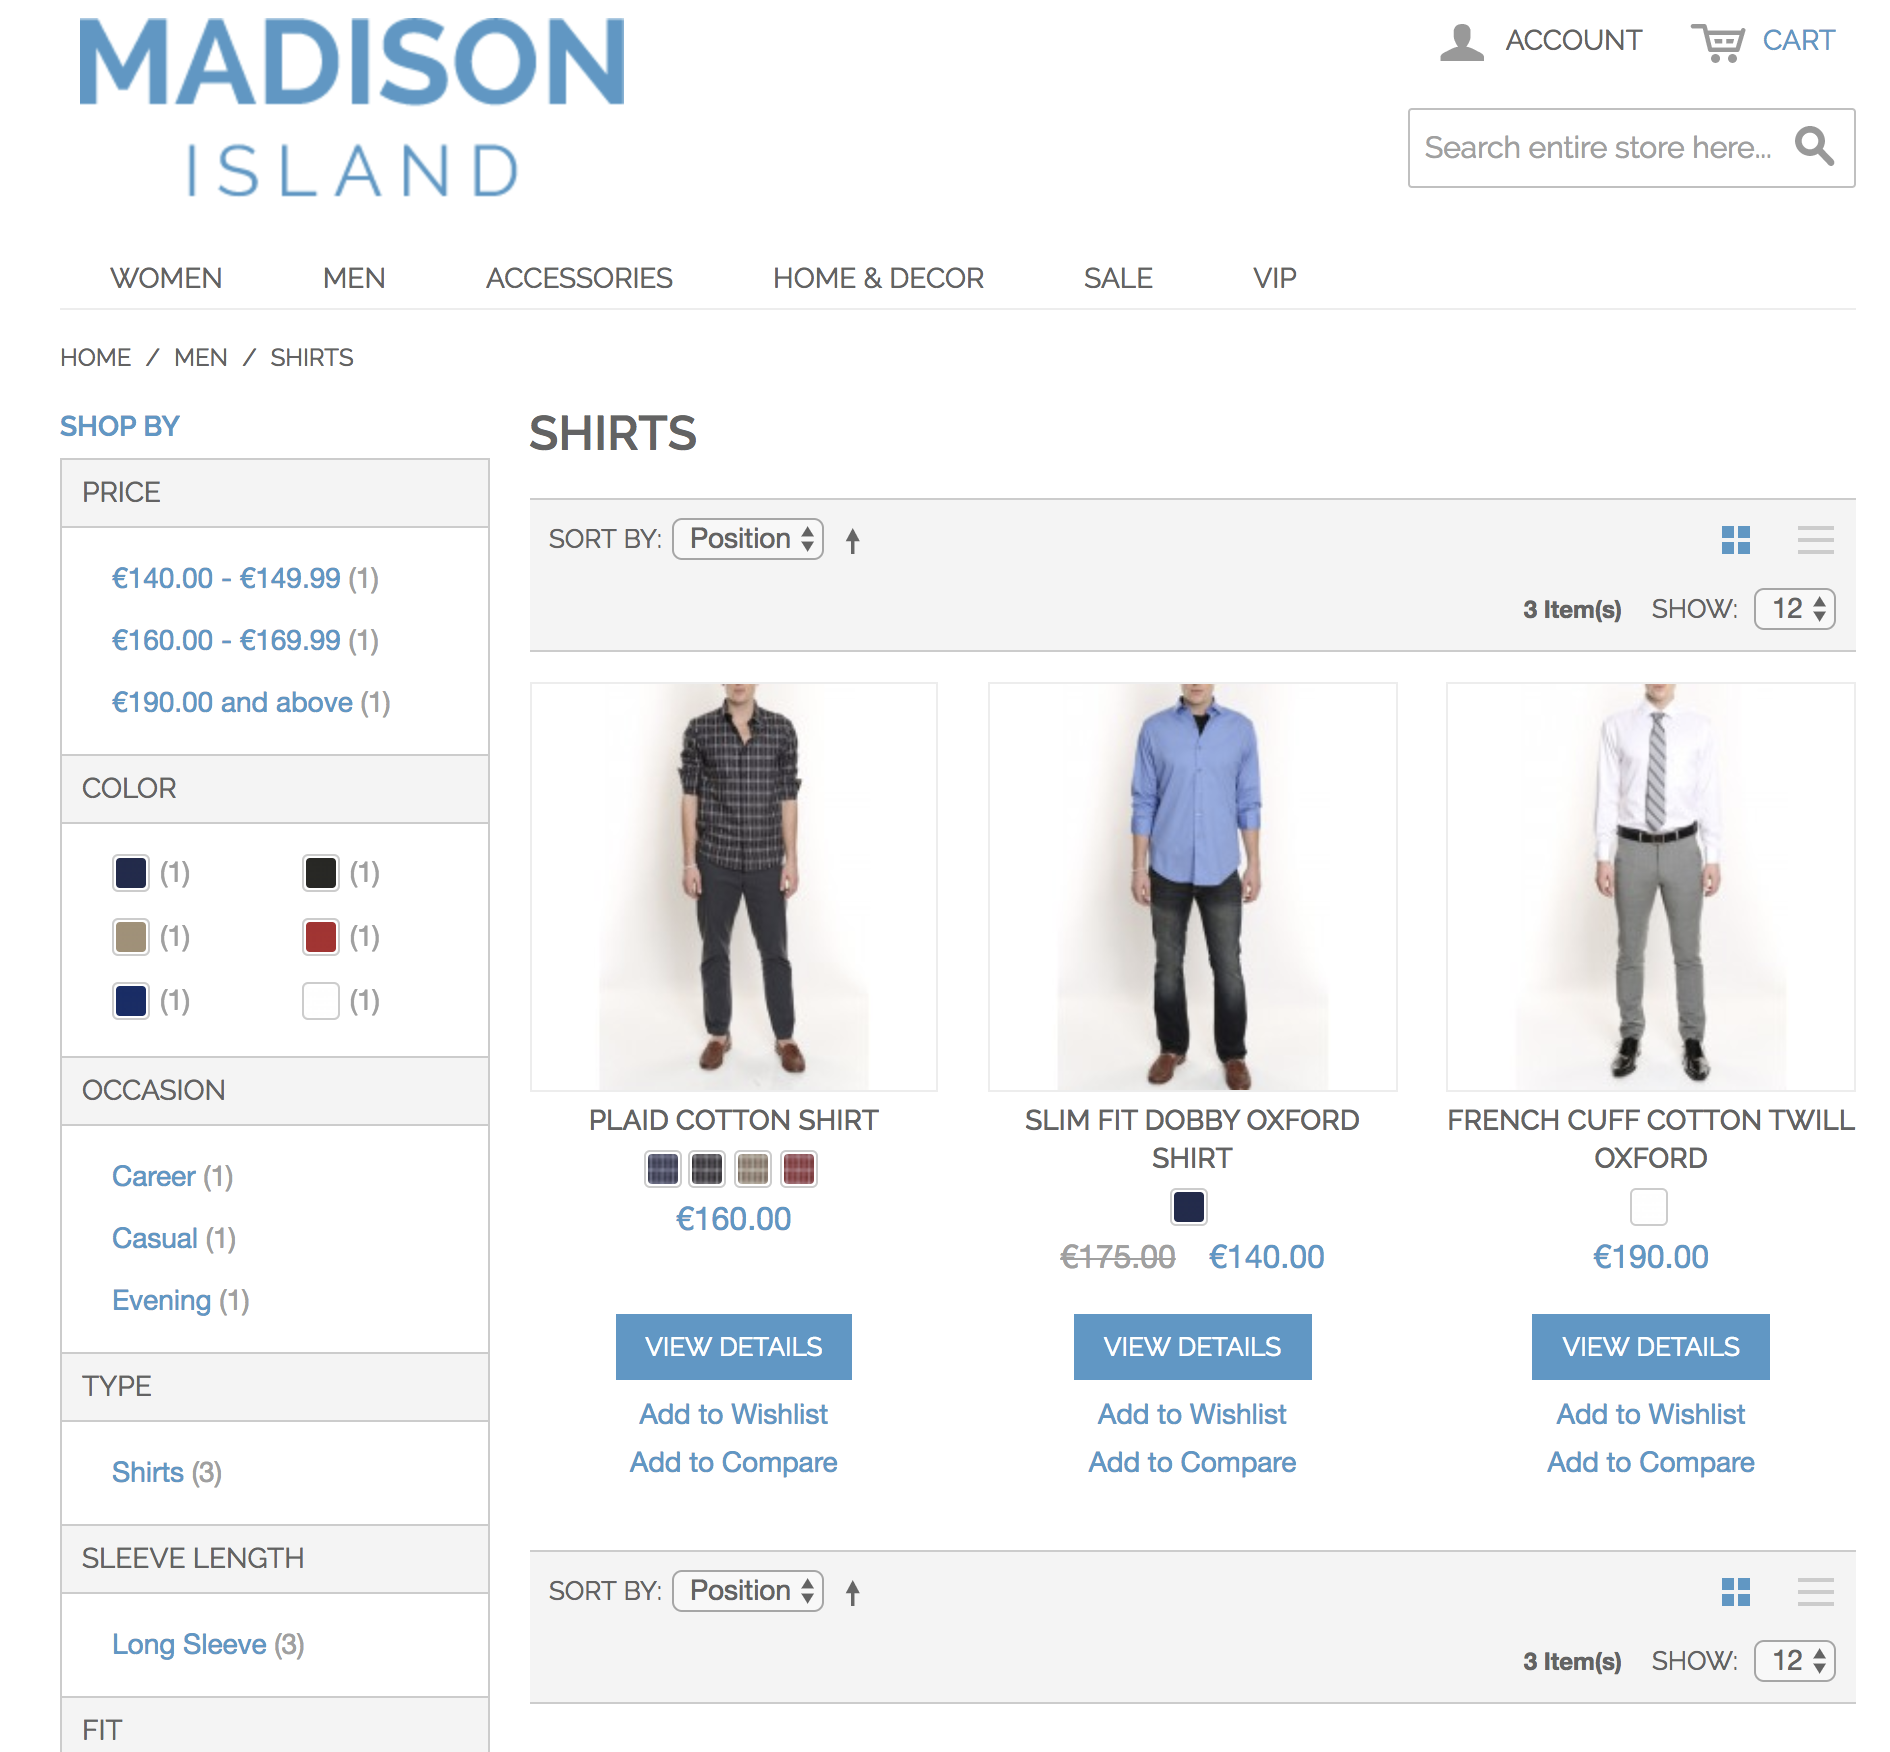
\includegraphics[width=7cm]{images/madison/products-list.png} }}%
  \caption{Different category page view modes}%
  \label{fig:category-display-modes}%
\end{figure}
\vspace{0.1cm}

Finally, from the product listing screen, the user can access any of the product detail pages clicking on the call to action \textit{te"View Details"} below the selected product image thumbnail. (Figure \ref{fig:product-detail})

\vspace{0.1cm}
\begin{figure}[H]
  \centering
    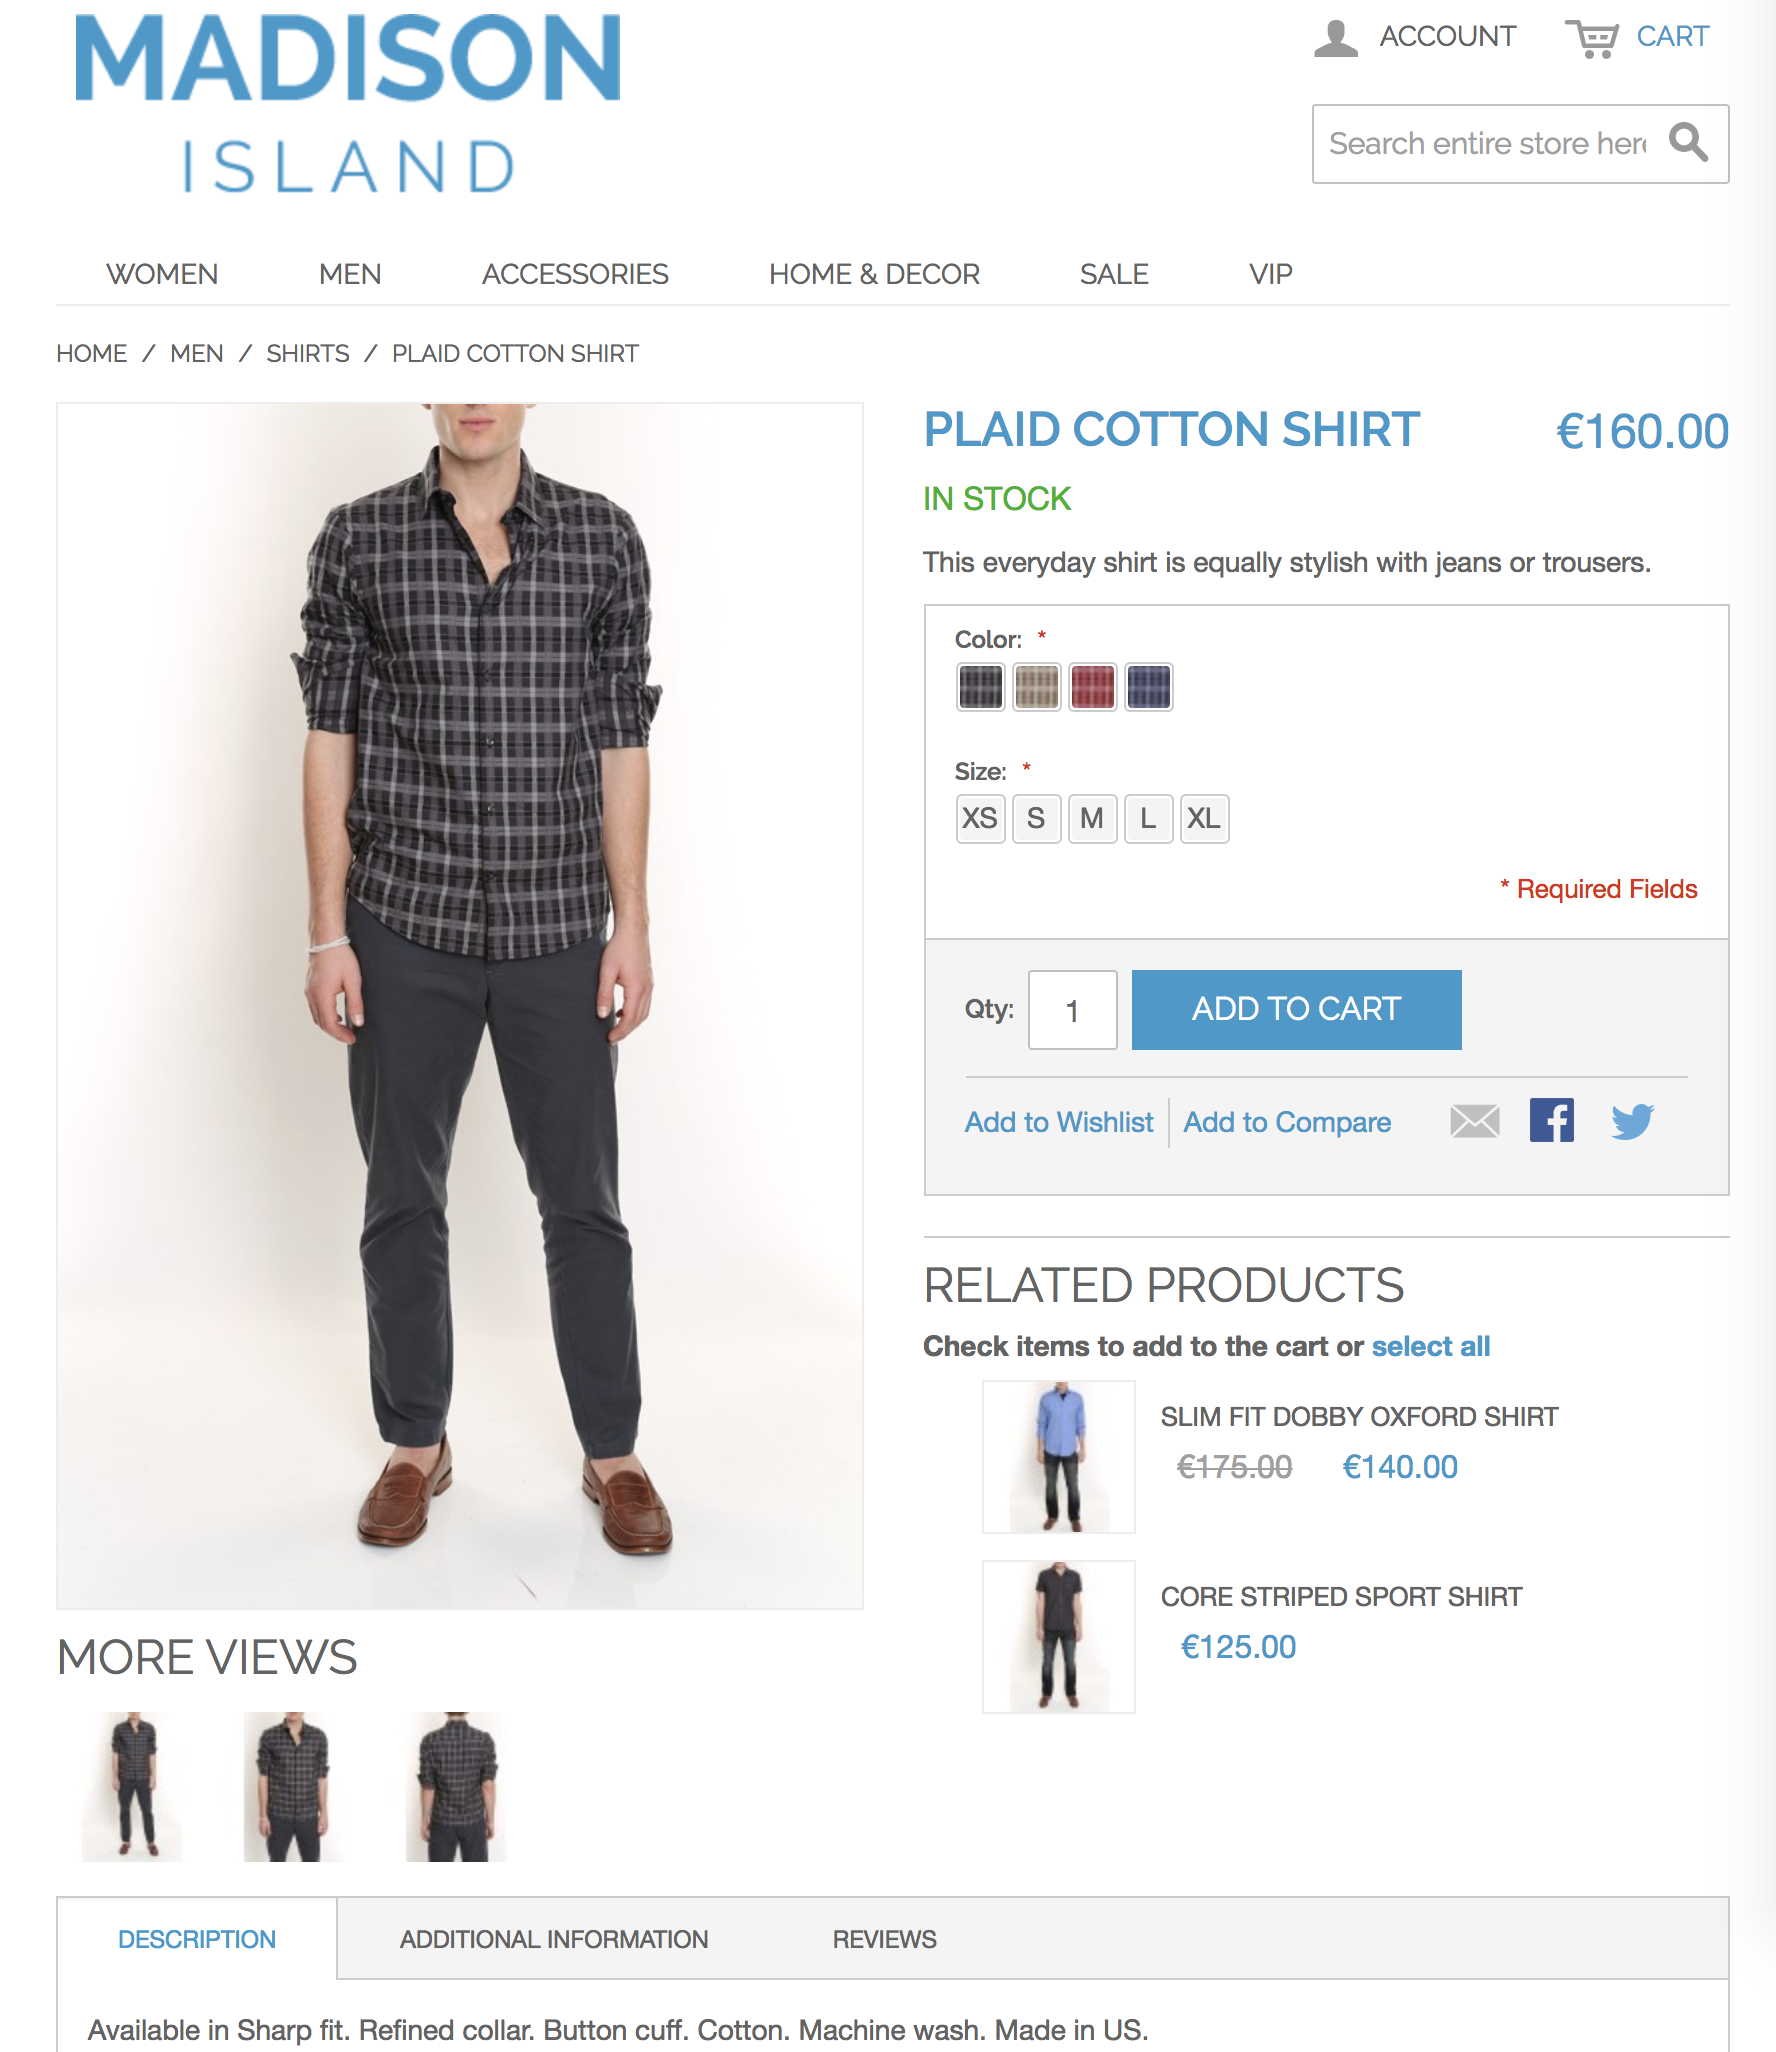
\includegraphics[height=8cm]{images/madison/product-detail.png}
  \caption{Product detail page}
  \label{fig:product-detail}
\end{figure}
\vspace{0.1cm}

The end to end interaction from the homepage to the product detail page can be represented with a model using the following IFML notation:

\vspace{0.1cm}
\begin{figure}[H]
  \centering
    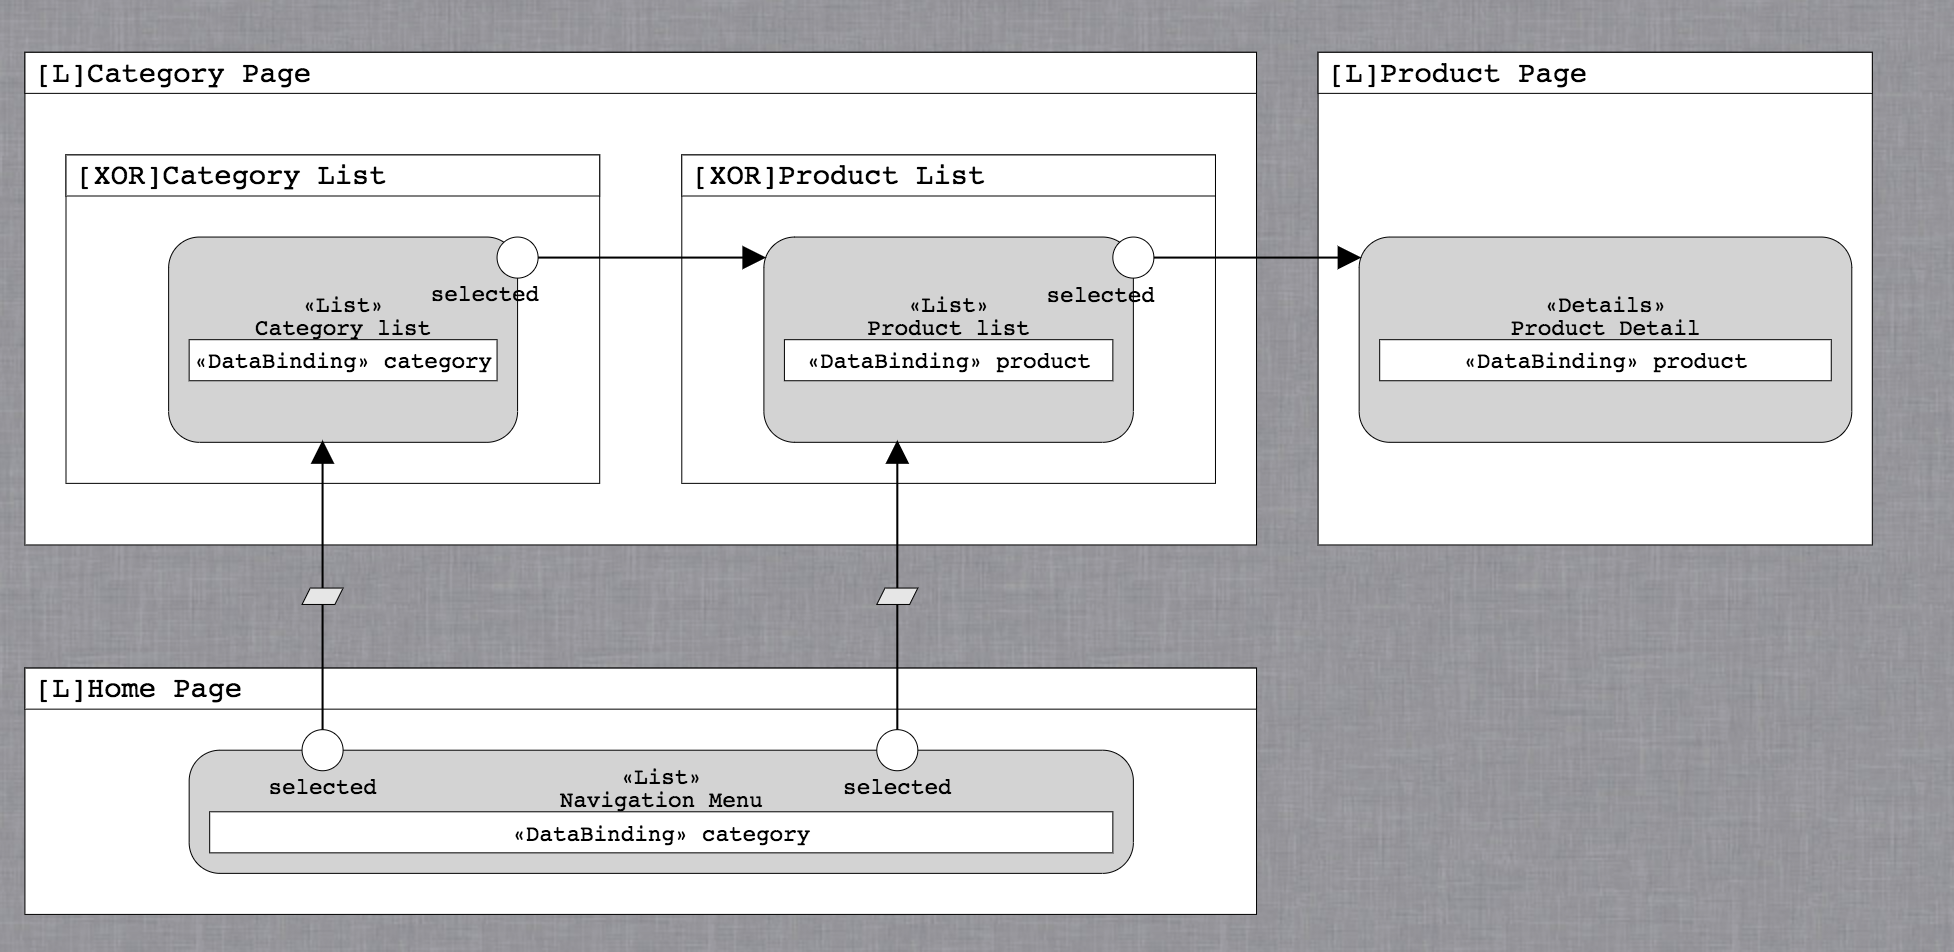
\includegraphics[width=12cm]{images/madison/ifml1.png}
  \caption{IFML representation of the Product Detail interaction}
  \label{fig:ifml1}
\end{figure}
\vspace{0.1cm}

The very same interaction can be expressed as a stream of records in the application server access logs which aim is to track all the requests processed by the web platform. Here's an example of  the very same user journey we just outlined above :

\begin{center}
  \begin{tabular}{|l|c|p{6cm}|}
  \hline
  \multicolumn{3}{|c|}{Application Server Access Log}\\ \hline
  \textbf{Page ID}&\textbf{IFML View Container}&\textbf{Log Entry}   \\ \hline
  Home Page&Home Page&\em[29/Nov/2017:06:30:45 +0000] "GET /" 200 0 - 29505 \\ \hline
  \textit{"View All Men"} Category&Category List&\em[29/Nov/2017:06:49:38 +0000] "GET /men.html 200 0 - 29505 
  \\ \hline
  \textit{"Shirts"} Category &Product List&\em[29/Nov/2017:07:04:15 +0000] "GET /men/shirts.html" 200 0 - 29505
  \\ \hline
  \textit{"Plaid Cotton Shirt"} Product &Product Page&\em[29/Nov/2017:07:08:40 +0000] "GET /men/shirts/plaid-cotton-shirt-476.html" 200 0 - 29505
  \\ \hline
  \end{tabular}
  \end{center}

\subsection{Products association and correlation}

In this scenario, we analyze the set of actions that can possibly generate page views among different product pages on the Madison Island website. 

Using as a starting point the same product page for the "Plaid Cotton Shirt" article of the previous navigational behavior analysis,the customer is presented with a \textit{"Related Products"} widget just below the \textit{"Add To Cart"} segment. The principal purpose of this section is to provide the user with some suggestions about products that can be linked in some way to the current one and generate customer's interest.(Figure \ref{fig:related-products})

\vspace{0.1cm}
\begin{figure}[H]
  \centering
    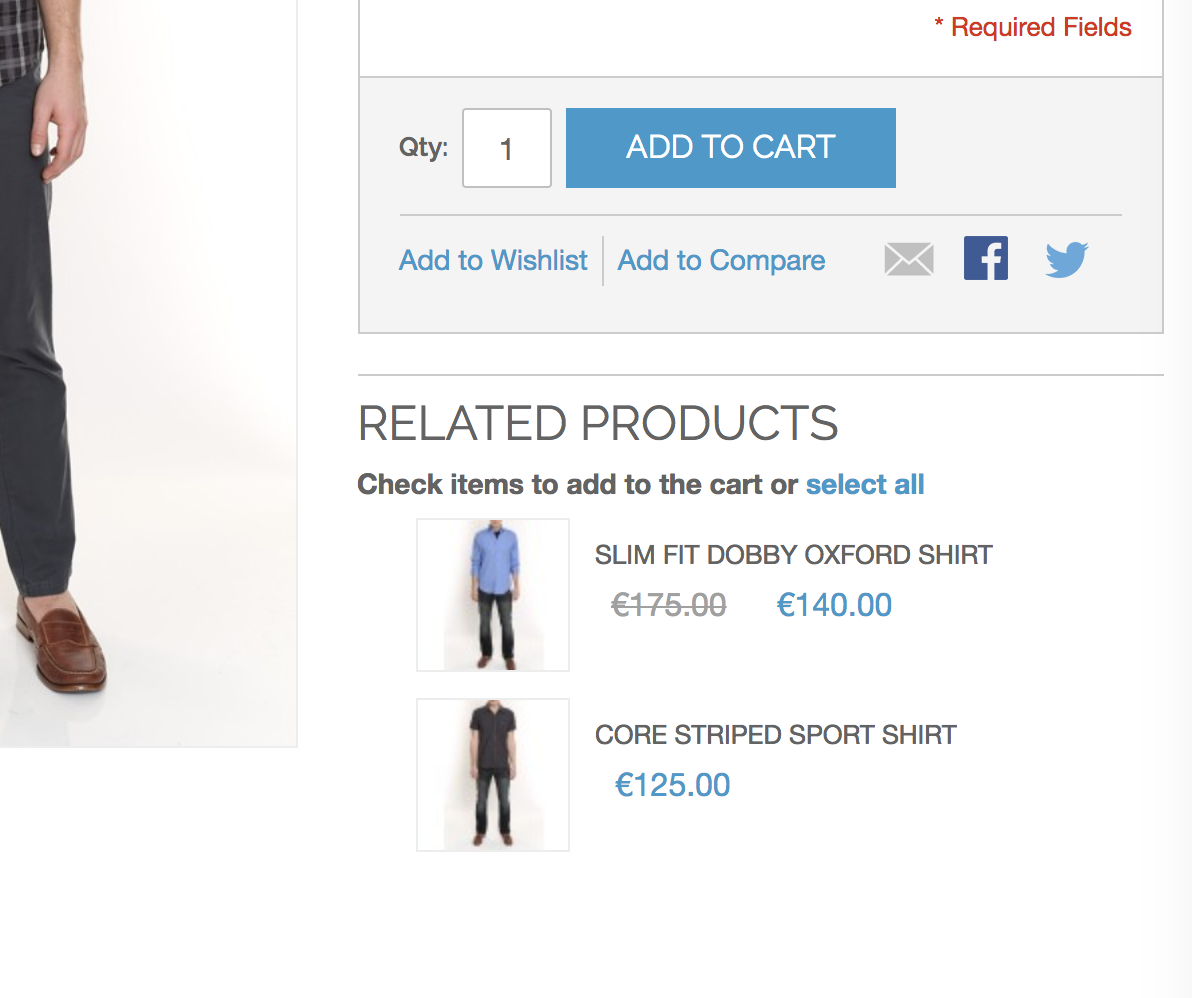
\includegraphics[width=8cm]{images/madison/related-products.png}
  \caption{Related products section}
  \label{fig:related-products}
\end{figure}
\vspace{0.1cm}



\section{IoT behavioral modeling}






\section{Analysis and Pattern recognition}



